\documentclass[12pt, letterpaper, twoside]{article}
\usepackage[utf8]{inputenc}
\usepackage{amsmath}
\usepackage{graphicx}
\usepackage{caption}
\usepackage{subcaption}
\usepackage{fancyref}


\title{Discussion on CAMs and GAPs}
\author{Marc, Fred, Nat, Isa \thanks{On a tous des prénoms à une syllabe comme ca ;)}}
\date{March 2017}

\begin{document}


	\begin{titlepage}
	\maketitle
	\end{titlepage}

	\section{Abstract}
	\label{sec:abstract}
	In this paper, we present both a novel VGG-GAP model inpired and benchmarked over a VGG-GAP-FC model introduced by \cite{zhou2016learning} and a regularization technique which increase the accuracy of our model and helps for both visualization and localisation of classes.
	
	In this work we further demonstrate the use of Global average pooling (as in \cite{zhou2016learning}) in conjunction with some regularizer in order to perform class localization. We also propose a modified version of the GAP network such that the network doesn't rely on any fully connected neurons. We evaluate our work on two datasets, the first one is an augmented version of the MNIST dataset\cite{lecun1998gradient} and the second one is the Stanford Actions 40 dataset\cite{yao2011human}. Comparing our technique with \cite{zhou2016learning}, we are able to enhance the overall class prediction and class localization on natural images drawn from actions 40. \\
	full image context awareness.


	\section{Introduction}
	\label{sec:introduction}
	The initial aim of this work is to evaluate the performance of a semi-supervised deep neural network for class localization in an image.
	The context is the following : its very easy to find a large amount of images labeled by name but harder to find large corpora of images labeled both by name and their localization. Based on this observation and on the work of Zhou at al. \cite{zhou2016learning}, whom proves that it's possible to extract a class localizations based on images only tagged by name, we propose to  further analysis of their models 

	\section{Our work}
	\label{sec:related_work}
	The way we structured our work is the following: at first we build two baselines, ConvFC is
	at first, we tested our hypothesis on two augmented versions of MNIST, then we tested the same methods on realistic images drawn from actions 40. As a base for comparison, we compare ourselves to a naive CNN followed by a FCNN and to the model proposed by Zhou at al. 

	\subsubsection{Model}
	\label{ssub:model}
	The model we use is a stack of convolutional layers ending with a Global Average Pooling Layer which averages are directly connected to the softmax function.
	

	\subsubsection{MNIST} 
	\label{ssub:mnist}
	The first 


	\section{Analysis}
	\label{sec:analysis}
	

	\section{Conclusion}
	\label{sec:conclusion}

	Reading through the literature, 2 interesting papers emerged. The first one, from Simonyan et al.\cite{simonyan2013deep} describe how back propagating the loss of image, through a convNet (like \cite{lecun1998gradient}), with respect to its input images can result in a saliency map. The second one, from Zhou et al.\cite{zhou2016learning}, put to evidence that a different network architecture using Convolutional layers followed by the GAP layer proposed by lin et al.\cite{lin2013network} and a fully connected layer could result in a proper semi-supervised learning of a class saliency visualized through a method they call CAM. Our paper is a follow up on this last one. We propose two methods to enhance the results retrieved by the model.

	The first method we propose is aimed at having (a) a better visualization of the Class Activation Mapping (CAM) and at (b) differentiating better one class from an other at the class activation level or, in other words, to build more specific CAM neurons.

	The second method slightly redefines the way one can use the GAP layer for semi-supervised learning of a class localization. 


	\subsection{model} 
	\label{sub:model}
		To test our first method, we train a VGG16 \cite{simonyan2014very} model as proposed by Zhou et al.\cite{zhou2016learning}, which is to say, we remove the the layers after conv5-3 and add a $3\times3$ convolutional layer of stride 1 with 1024 units, followed by a GAP layer, a fully connected layer with $N$ units ($N$ classes) and a softmax layer. We refer to this model as the 'VGG-CAM-FC'.
		Formally, the end of the network is defined as follows : lets $f_k(x,y)$ be the activation of unit $k$ in the last convolutional layer at the spatial location (x,y), then the Global Average Pooling is defined by :
		\begin{equation}
			\textrm{GAP}_k = \sum_{x,y} f_k(x,y)
		\end{equation}
		In this model, the GAP layer if fully connected to the softmax layer, therefore the prediction value for class 'c' ${p^c}$ is computed as follows:
		\begin{equation}
			p^c = \textrm{softmax}\left(\sum_{k} w^c_k \cdot \textrm{GAP}_k\right)
		\end{equation}
		We kindly remind here, that, because of this definition, the $\textrm{GAP}_k$ values are positions agnostic and that we recover the class saliency from the $f_k(x,y)$ and the $w^c_k$ values using a "Class Activation Mapping (CAM)" which is defined by : 
		\begin{equation}
			\textrm{CAM}^c(x,y) = \sum_k w^c_k \cdot f_k(x,y)
			\label{eq:GAP_FC_CAM}
		\end{equation}


		Corresponding to the thesis subject of the writer, this model has been trained and tested on the Stanford 40 actions dataset \cite{yao2011human}. This dataset is composed by 4000 training images of humans performing, on each images, one of 40 actions and 5532 testing images.
	
	\subsection{Analyzing the results of the original model}
	\label{sub:analyzing_original_model}
		We re-implemented the VGG model (as described earlier), which we named VGG-CAM-FC, trained it on the Stanford action 40, and achieved an accuracy of TODO : $51.6\%$. We then visualized the CAMs (e.g. \fref{fig:CAM_with_GAP_original}) and found that each of the individual 2D representations were not representative on their own. The values of the CAMs would only make sense in the context of all the others, and therefore, needed an extra processing to discriminate some classes one from the others. As one constrains of our work is to be able to extend our object saliency to a multi-class object saliency in a real-time framework, this original model was not practicable.
		\begin{figure}[h]
			\begin{subfigure}[c]{0.3\textwidth}
				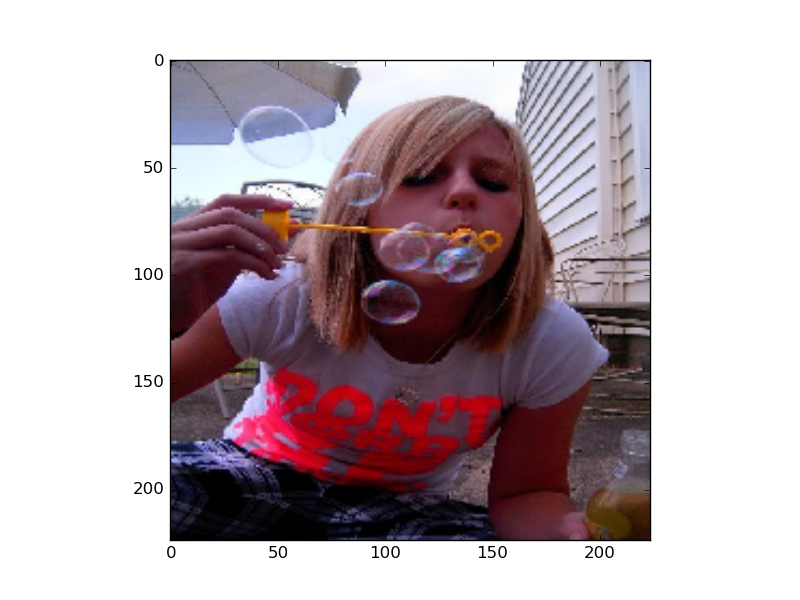
\includegraphics[width=\textwidth]{test_image}
			\end{subfigure}
			\begin{subfigure}[c]{0.69\textwidth}
				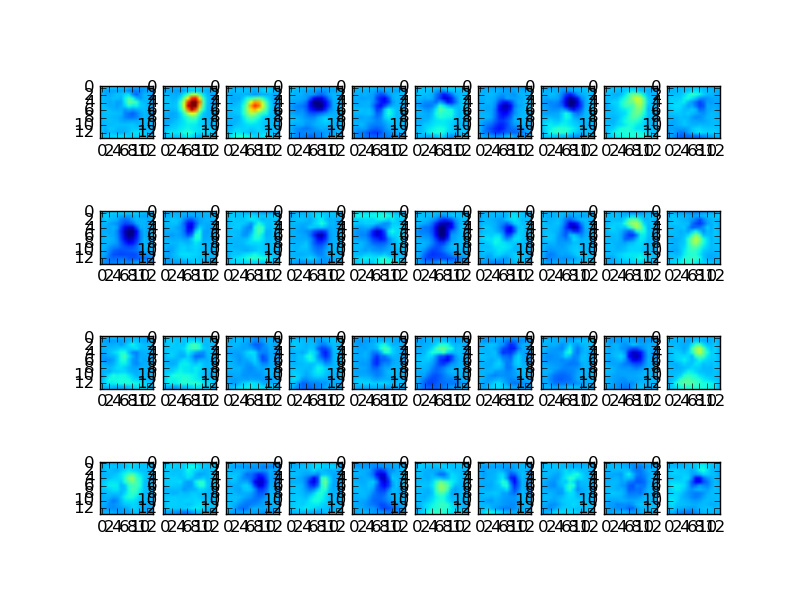
\includegraphics[width=\textwidth]{GAP_orig_viz}
			\end{subfigure}
			\centering
			\caption{On the left, a "blowing bubbles" testing images from Stanford 40 Action dataset. On the right, the CAM visualization of this image using the original model.}
			\label{fig:CAM_with_GAP_original}
		\end{figure}

	
	\subsection{Method one: Regularizing the CAM}
	\label{sub:regularizing_the_cam}
		To overcome this visualization issue we tried centering every $f_k(x,y)$ units around a single value. The intuition behind this move is to enforce the CAMs to be easily interpretable: at visualization time, the CAMs should depict many of this "center value" but where the class we predict is present. We found that zero would be a convenient reference. As a result, we expect to be able to discriminate when a class is highly probable and know where it stands when visualizing the CAM maps, without any processing , thank to a sparser representations.

		To render such properties on our model, we added either an L1 or an L2 regularization term in the resulting matrix of the last convolutional layer $f_k(x,y)$.
		\begin{equation}
			\begin{aligned}
				L_1 &= \alpha \sum_{x,y,k} |f_k(x,y)| \\
				L_2 &= \alpha \sqrt{\sum_{x,y,k} f_k(x,y)^2}
			\end{aligned}
		\end{equation}
		We chose the $\alpha$ value following a dichotomy method reducing this value by a factor of 10 until finding significant results. We also acknowledge here that it would be more rigorous, for generalization purposes, to compute this $\alpha$ value as a factor of the expected loss of the model.

		\vskip .5em
		\textbf{Accuracy results:}\\
		The first results we can appreciate are the different accuracies, precision and recall values of the models. On the one hand, it was expected the precision will increase in the regularized models as they should have a better discrimination factor caused by shrinking all the neurons values around zero but, on the other hand, it was unexpected that the accuracies would raise. TODO : COMMENTER LA DIFF (APRES UPDATE DES VALEURES)

		\begin{center}
			\begin{tabular}{ |c|ccc| }
				\hline
				Model & VGG-GAP-FC & VGG-GAP-FC & VGG-GAP-FC \\
				& & ($L_1$: $\alpha=.7$) & ($L_2$: $\alpha=.7$) \\
				\hline
				Accuracy & 51.6\% & 59.2\% & 61.5\% \\
				Precision & 60.1\% & 71.1\% & 80.9\% \\
				Recall & 47.6\% & 52.0\% & 47.4\% \\
				\hline
			\end{tabular}
			TODO : LES RESULTATS VONT CHANGER (AU MOINS 57\% D'ACCURACY SUR LE PERMIER MODEL)(RE-CALCUL CETTE NUIT)
		\end{center}


		\vskip .5em
		\textbf{CAMs results:}\\
		When we visualize the CAMs, there is less ambiguity or more visual clues about which CAM depict a localized class. REDESSINER CA...
		\begin{figure}[h]
			\begin{subfigure}[t]{0.32\textwidth}
				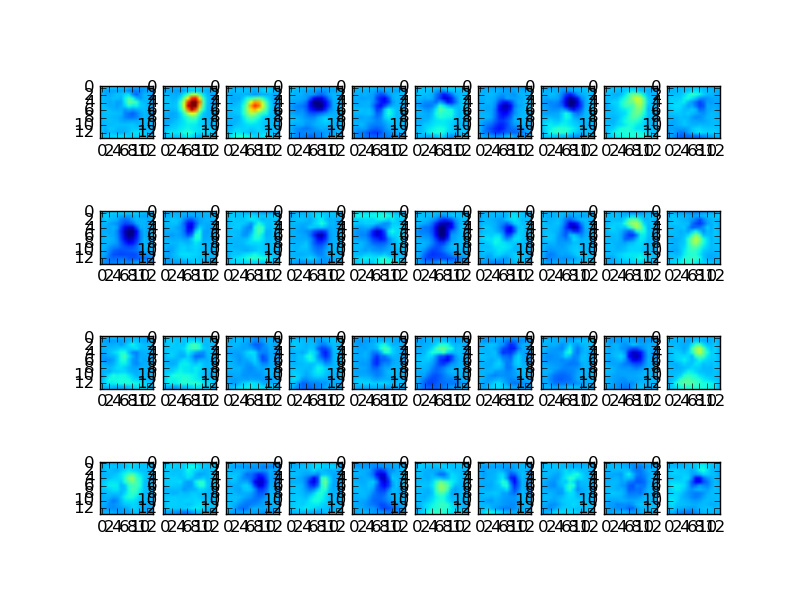
\includegraphics[width=\textwidth]{GAP_orig_viz}
				\caption{VGG-GAP-FC}
			\end{subfigure}
			\begin{subfigure}[t]{0.32\textwidth}
				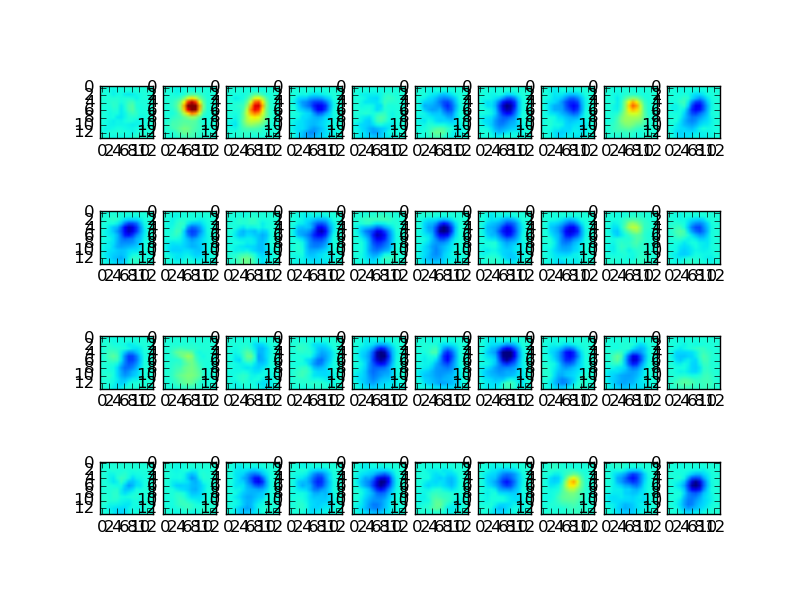
\includegraphics[width=\textwidth]{GAP_orig_L1_1e7}
				\caption{VGG-GAP-FC \\($L_1$: $\alpha=.7$)}
			\end{subfigure}
			\begin{subfigure}[t]{0.32\textwidth}
				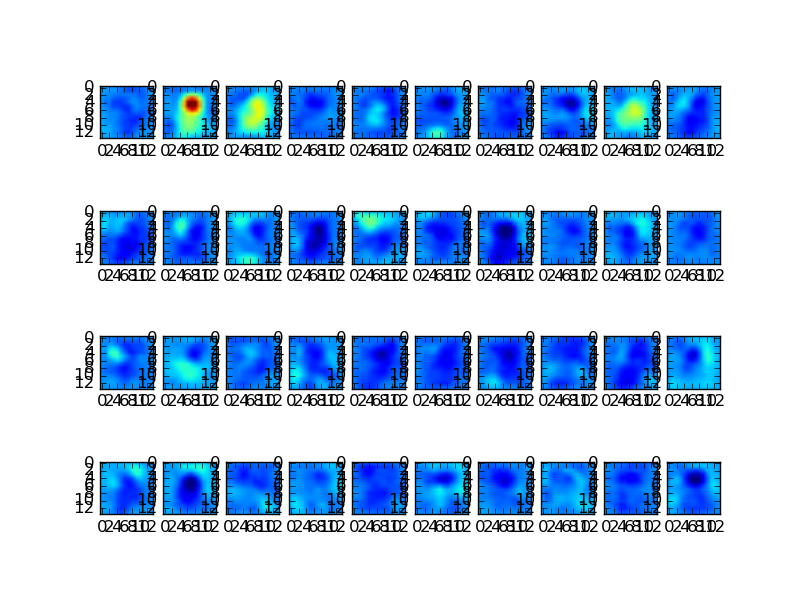
\includegraphics[width=\textwidth]{GAP_orig_L2_1e7}
				\caption{VGG-GAP-FC \\ ($L_2$: $\alpha=.7$)}
			\end{subfigure}
			\centering
			\caption{Visualization of the CAM values, as defined in equation \ref{eq:GAP_FC_CAM}, for every one of the 40 classes for the same model trained with different regularization parameters.}
			\label{fig:CAM_with_GAP_original_regularized}
		\end{figure}

		\vskip .5em
		\textbf{Activations values:}\\
		Finally, \fref{fig:GAP_orig_regularized_activations} shows how the activation values changed from one training to the other. We notice that the $L_1$ trained model have a similar looking activation distribution than the original model that is only shifted and rescaled. Whereas the $L_2$ trained models have very different properties. (a) Most of the activation values are now shrank to a value ranging between -2 and +2 and (b) the values over 2 (human observation) are potential candidates for the class.
		\begin{figure}[h]
			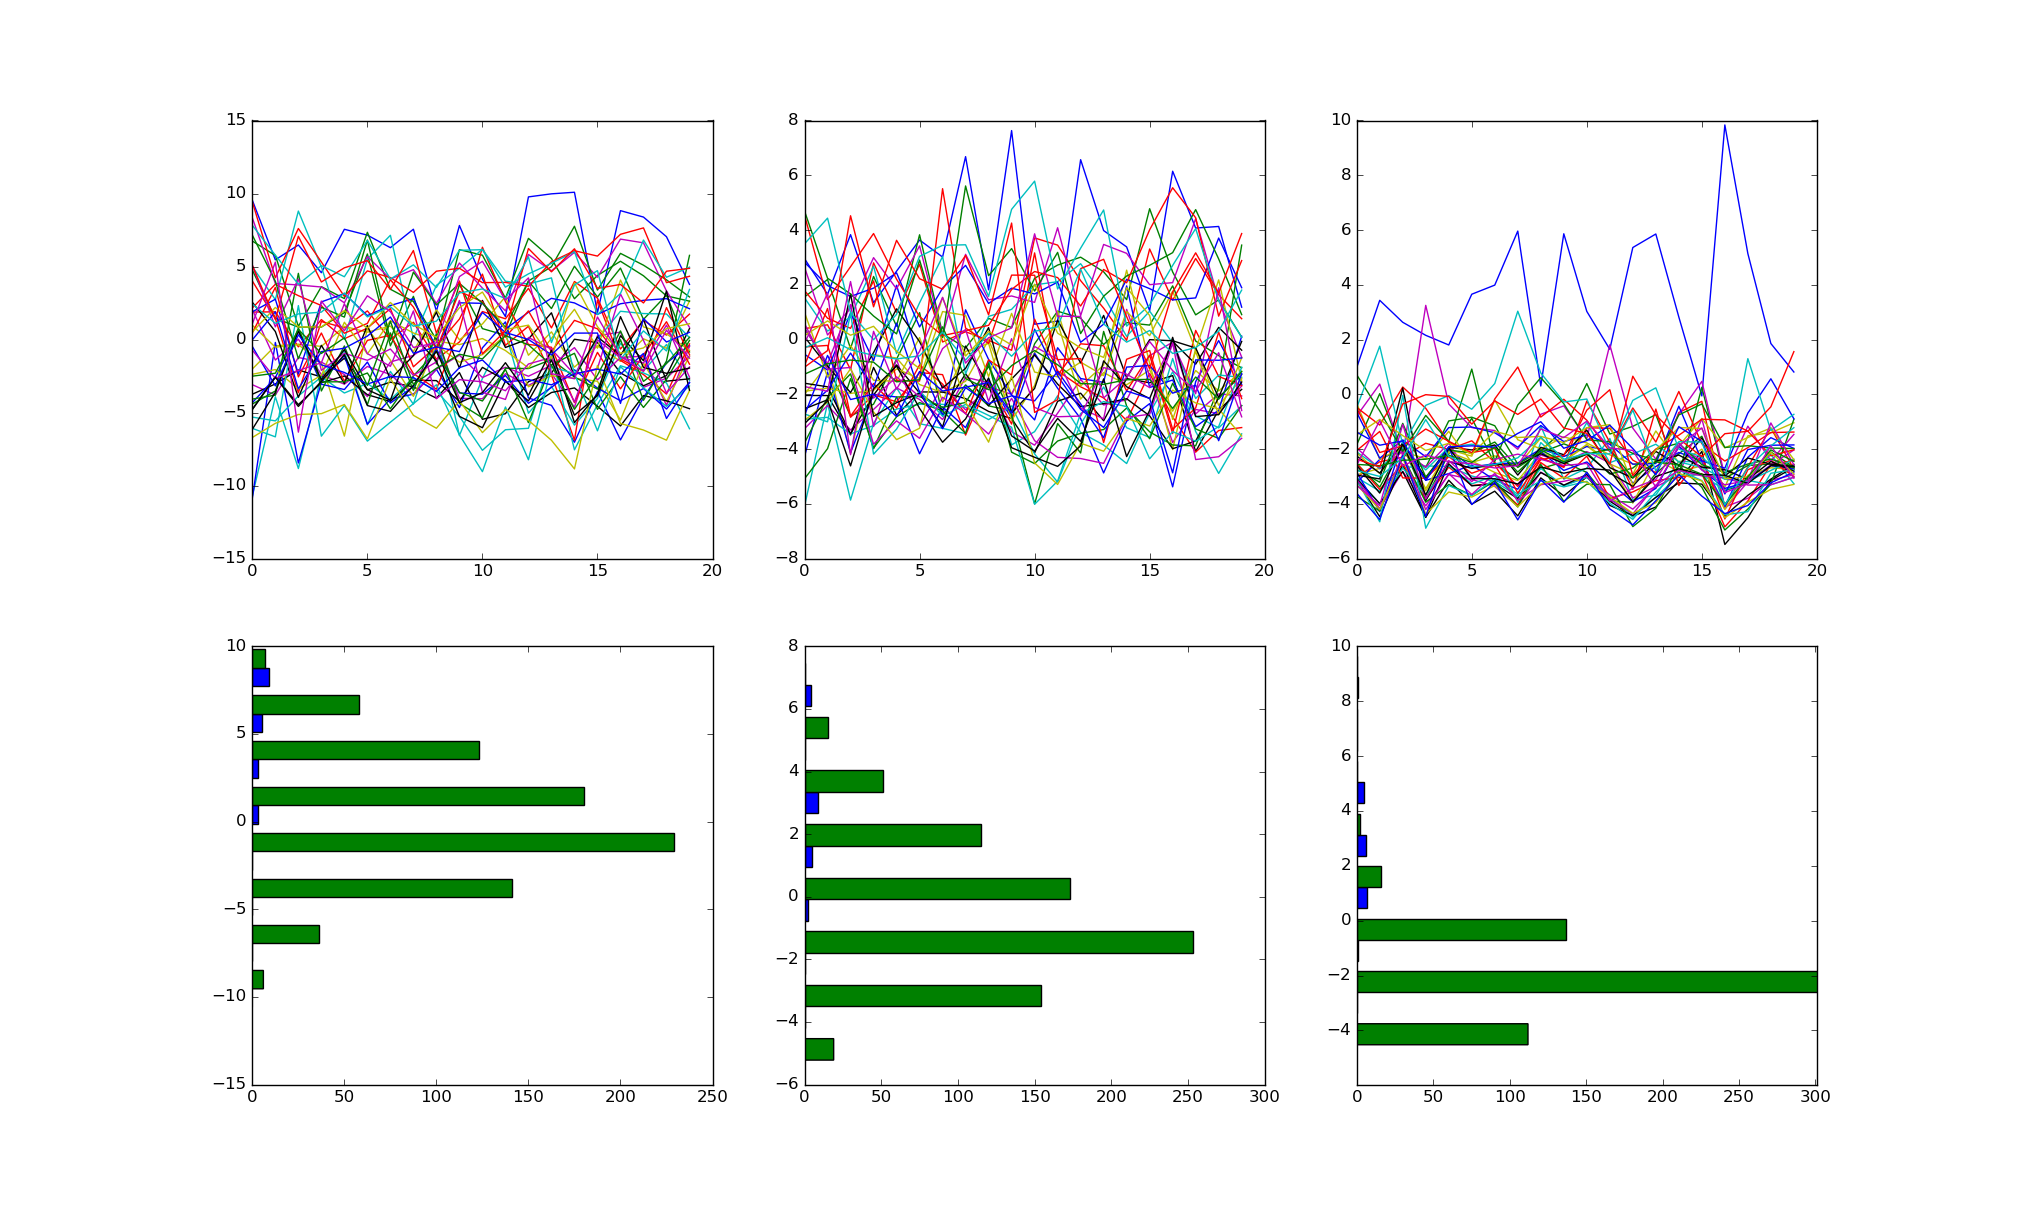
\includegraphics[width=\textwidth]{GAP_orig_activations}
			\caption{ The six plots show, from left to right, results of VGG-CAM-FC, VGG-GAP-FC ($L_1$: $\alpha=.7$) and VGG-GAP-FC ($L_2$: $\alpha=.7$). Then, the top line (a) shows, in the vertical axes, the activations of the 40 neurons before the softmax layer and, on the y axis, the index of an image sampled in the test-set. \\
			We elected images that were correctly classified by another classifier to increase the probability of these three models to classify correctly too. \\
			And on the bottom line (b) the repartition of the activations of the neurons with, in blue, the activation of the true class and, in green, the activation of the other classes.}
			\label{fig:GAP_orig_regularized_activations}
		\end{figure}














	\subsection{Method two: Revisiting the original model}
	\label{sub:new_model}
		After seeing these results we experimented another model which would be fully defined by its spatial dependences. What we imply here is that the original VGG-CAM-FC model depended on a fully connected layer which allowed the model to separate a concept into two $f_k$ units which would not be spatially dependent whereas our model (on its first form)n can't. All the activations seen on our CAM can only depend on the given $(x,y)$ couple.

		to have dependencies which would not be spatially defined. In other terms the original model had the possibility to learn a dependency between two elements being present in an image but not being properly placed whereas our model cant generalize this property if it hasn't seen two elements in a particular position in a training set.



		\vskip .5em
		\textbf{Accuracy results:}\\

		\begin{center}
			\begin{tabular}{ |c|cccc| }
				\hline
				Model & VGG-GAP1 & VGG-GAP1 & VGG-GAP5 & VGG-GAP5 \\
				& ($L_1$: $\alpha=.7$) & ($L_2$: $\alpha=.7$) & ($L_1$: $\alpha=.7$) & ($L_2$: $\alpha=.7$) \\
				\hline
				Accuracy & 60.5\% & 60.5\% & 58.5\% & 60.0\% \\
				Precision & 718.\% & 83.9\% & 74.8\% & 91.4\% \\
				Recall & 48.0\% & 55.1\% & 27.2\% & 49.3\%  \\
				\hline
			\end{tabular}
		\end{center}


		\vskip .5em
		\textbf{CAMs results:}\\
		When we visualize the CAMs, there is less ambiguity or more visual clues about which CAM depict a localized class. REDESSINER CA...
		% \begin{figure}[h]
		% 	\begin{subfigure}[t]{0.32\textwidth}
		% 		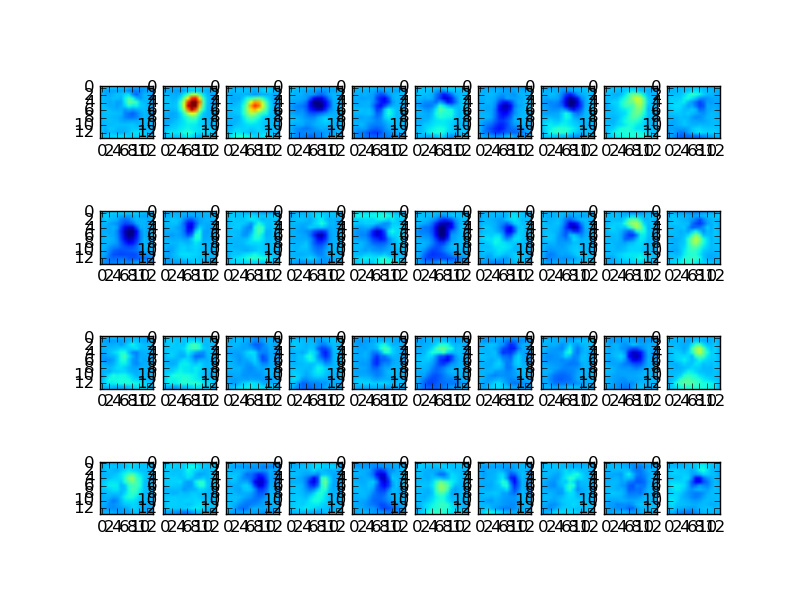
\includegraphics[width=\textwidth]{GAP_orig_viz}
		% 		\caption{VGG-GAP-FC}
		% 	\end{subfigure}
		% 	\begin{subfigure}[t]{0.32\textwidth}
		% 		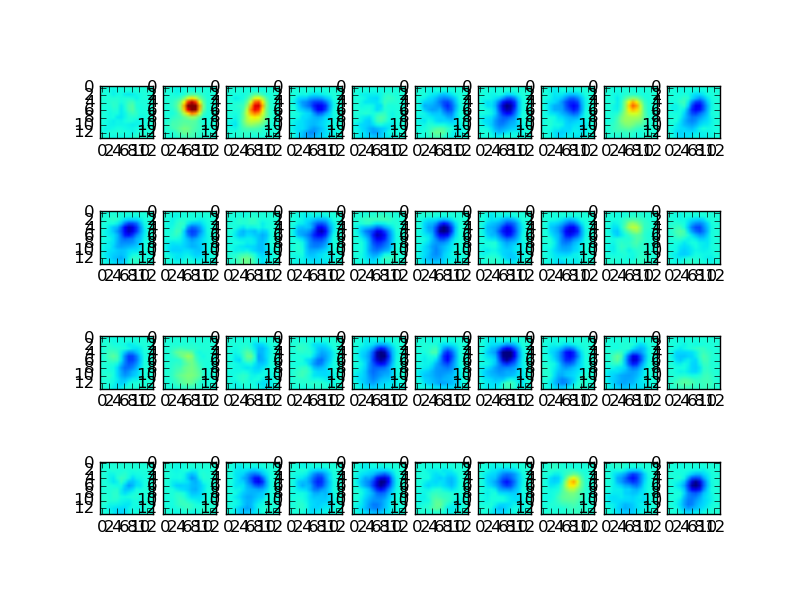
\includegraphics[width=\textwidth]{GAP_orig_L1_1e7}
		% 		\caption{VGG-GAP-FC \\($L_1$: $\alpha=.7$)}
		% 	\end{subfigure}
		% 	\begin{subfigure}[t]{0.32\textwidth}
		% 		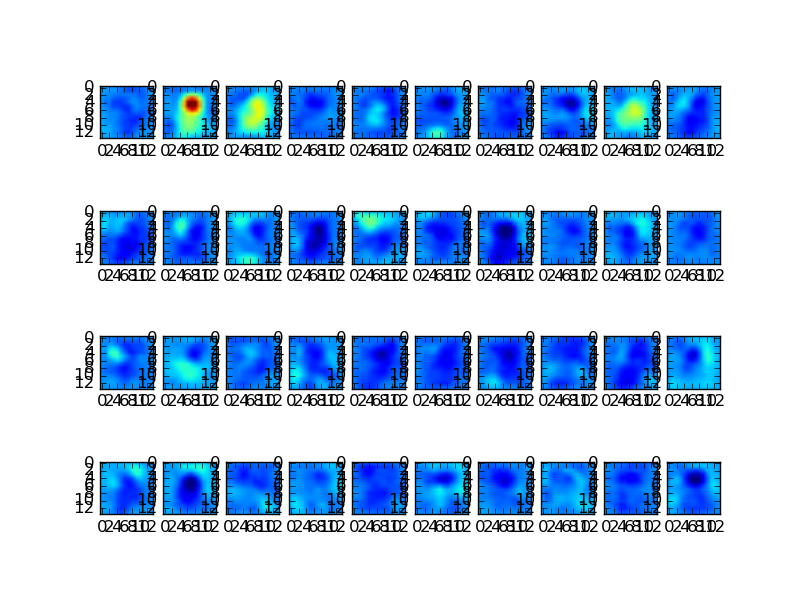
\includegraphics[width=\textwidth]{GAP_orig_L2_1e7}
		% 		\caption{VGG-GAP-FC \\ ($L_2$: $\alpha=.7$)}
		% 	\end{subfigure}
		% 	\centering
		% 	\caption{Visualization of the CAM values, as defined in equation \ref{eq:GAP_FC_CAM}, for every one of the 40 classes for the same model trained with different regularization parameters.}
		% 	\label{fig:CAM_with_GAP_original_regularized}
		% \end{figure}

		\vskip .5em
		\textbf{Activations values:}\\
		Finally, \fref{fig:GAP_orig_regularized_activations} shows how the activation values changed from one training to the other.
		\begin{figure}[h]
			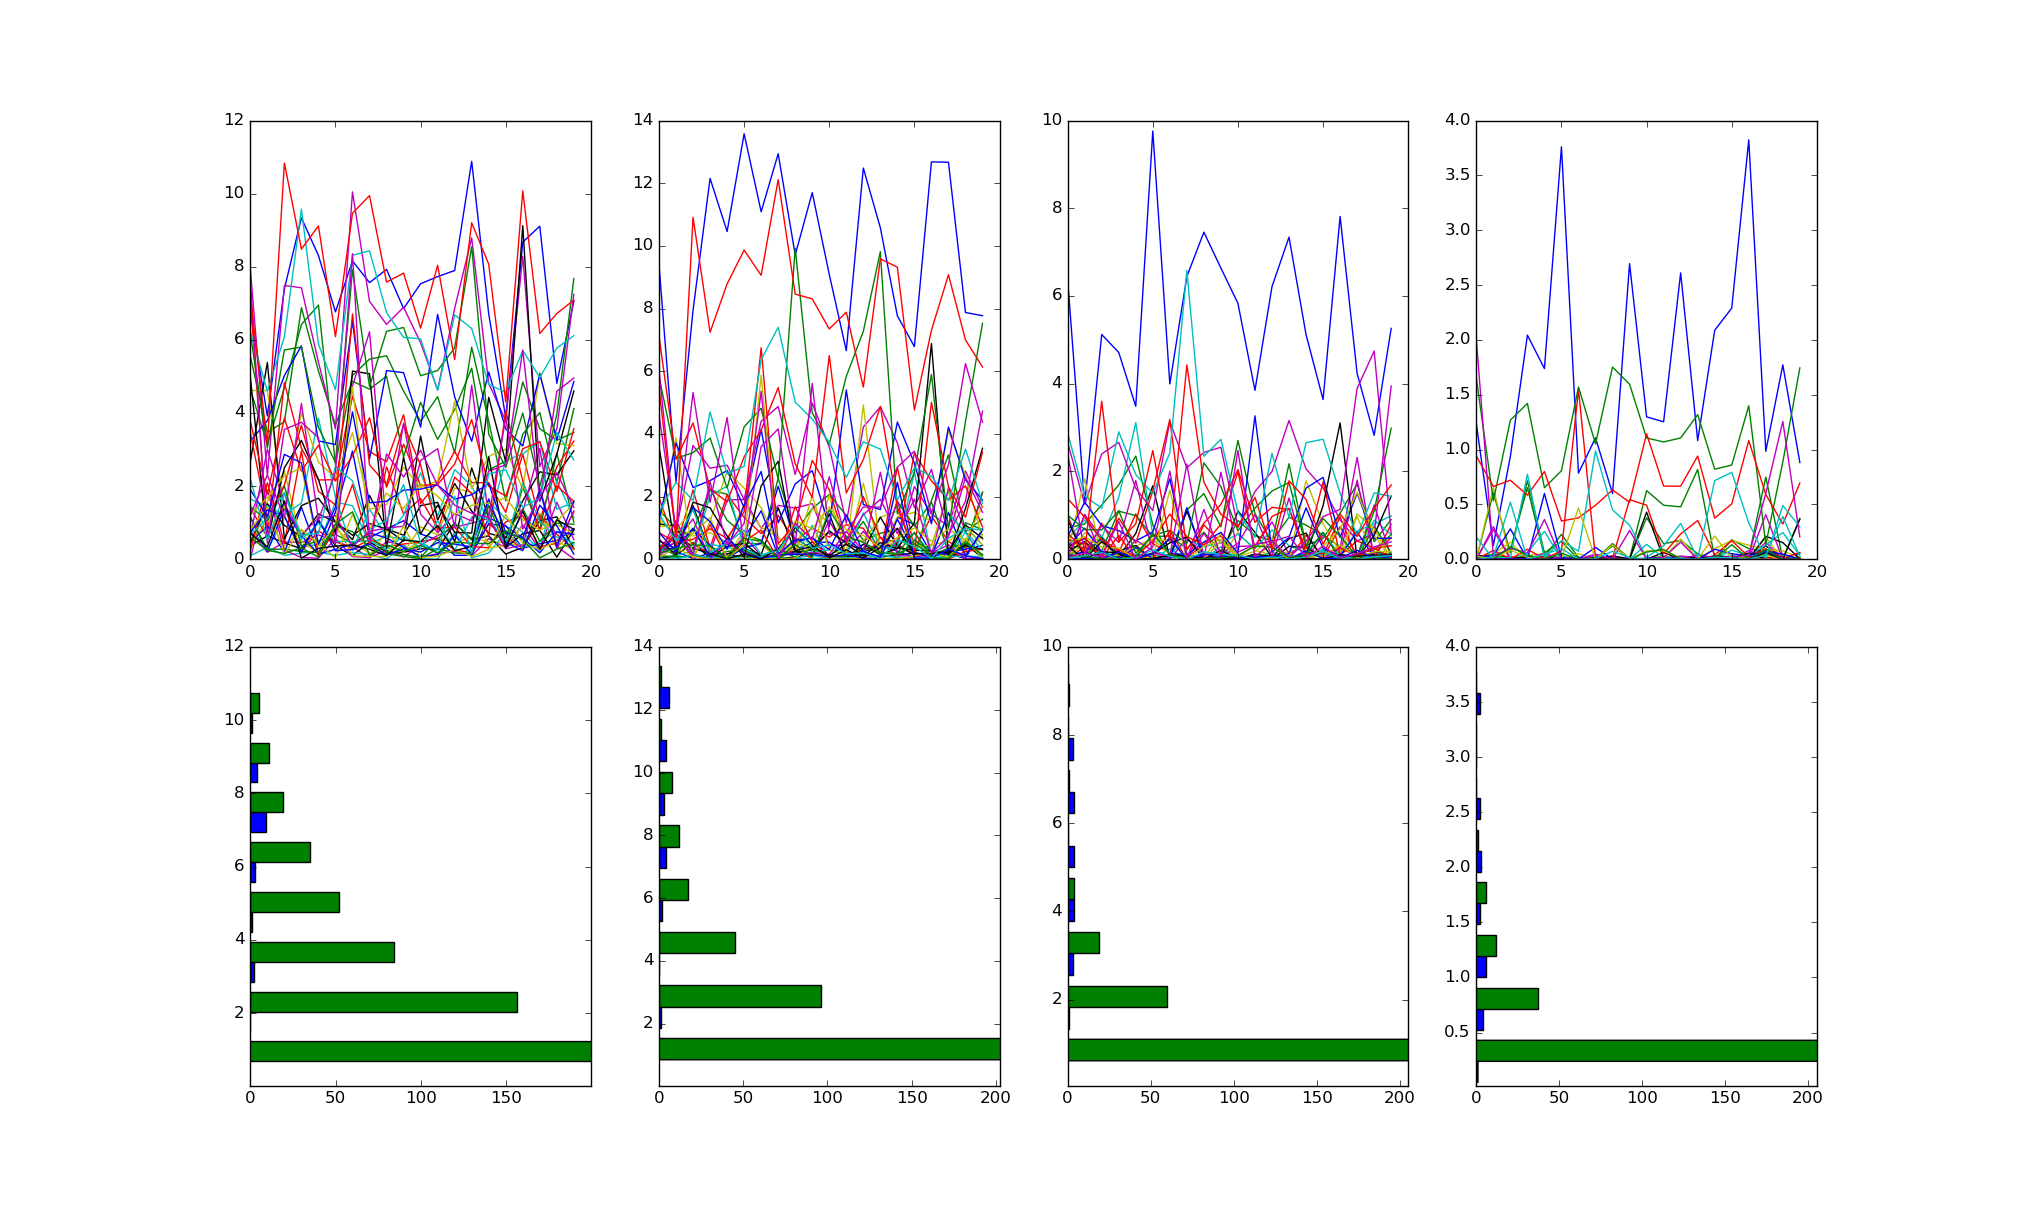
\includegraphics[width=\textwidth]{GAP1_activations}
			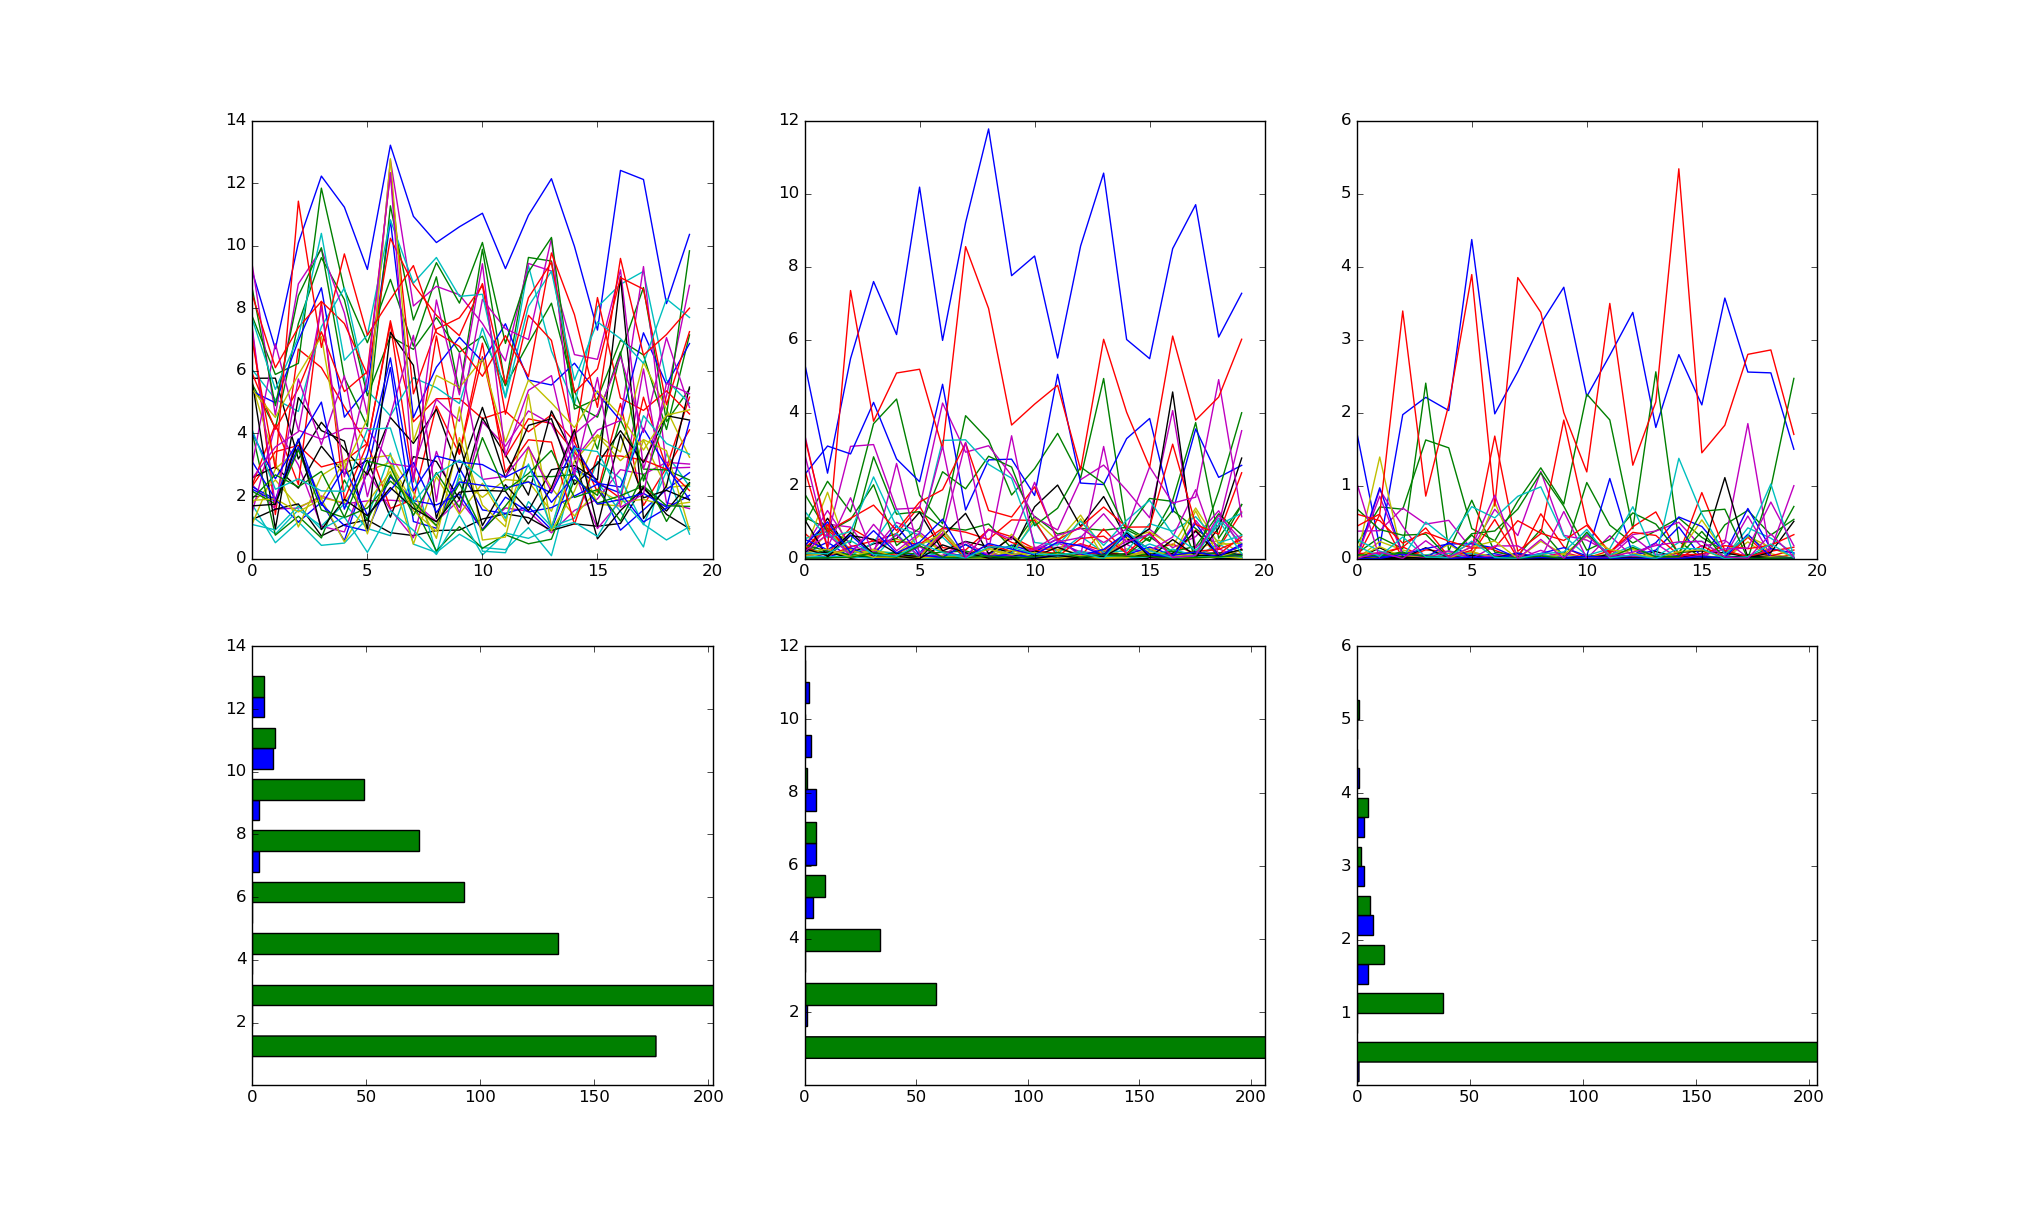
\includegraphics[width=\textwidth]{GAP5_activations}
			\caption{ }
			\label{fig:GAP_orig_regularized_activations}
		\end{figure}




\newpage
\bibliography{main}
\bibliographystyle{ieeetr}




\end{document}